\documentclass[11pt]{article}
\usepackage{enumitem}
\usepackage{amsmath,amsthm,amssymb}
\usepackage{color}
\usepackage{graphicx}
\graphicspath{ {./images/} }

\begin{document}
\date{} 
\title{Lab Report 2\\--\\\large CPE282 Fall 2020}
\author{Brennen Green}
\maketitle

\section*{Display Driver}
\begin{center}
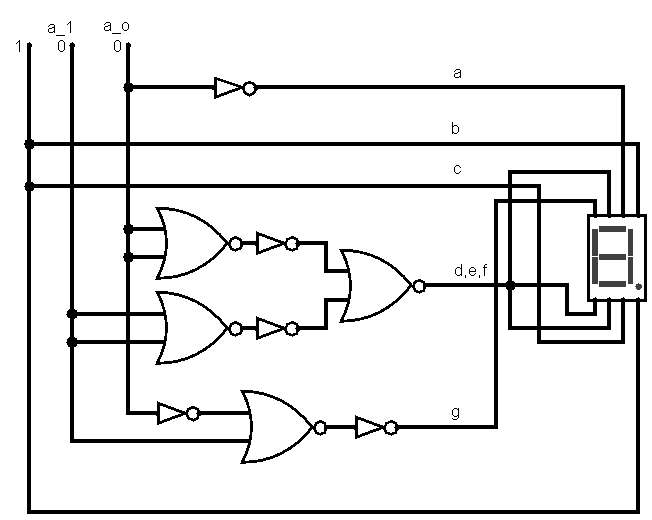
\includegraphics[width=10cm, keepaspectratio]{DisplayDriver}\newline
\end{center}
This design had a couple of road bumps during the implementation. Firstly, I misunderstood the use of the 74LS04 chip for inverting signals. Actually, I didn't use the chip at all.
While this had no effect on the output of my design, it did make setting up my design a bit harder and more redundant as a I had to use the quad input NOR gate chip to invert signals which
made wiring up my design pretty problematic. None the less, I followed my prelab design pretty spot on and despite these mishaps it worked well.
\section*{Custom Priority Encoder}
\begin{center}
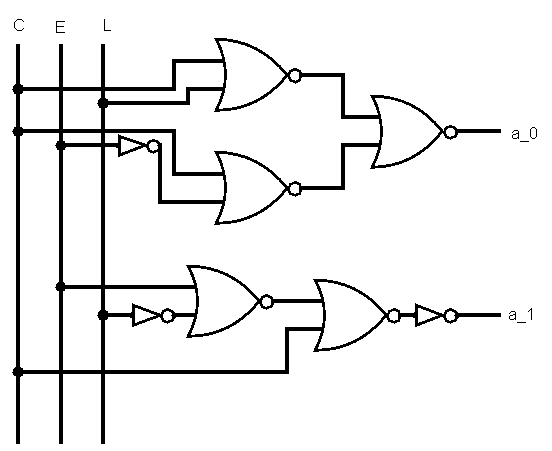
\includegraphics[width=10cm, keepaspectratio]{Encoder}\newline
\end{center}
This implementation went a lot smoother. For one, I did (with the help of my lab TA) discover the use of the 74LS04 chip which made inverting signals a lot easier and wiring a lot less of a pain.
However, this design did slightly vary from the design in my prelab. With my prelab, I made an error in designing the output circuit for $a_0$, that error was corrected in this final design.
\newpage
\section*{Final Design}
\begin{center}
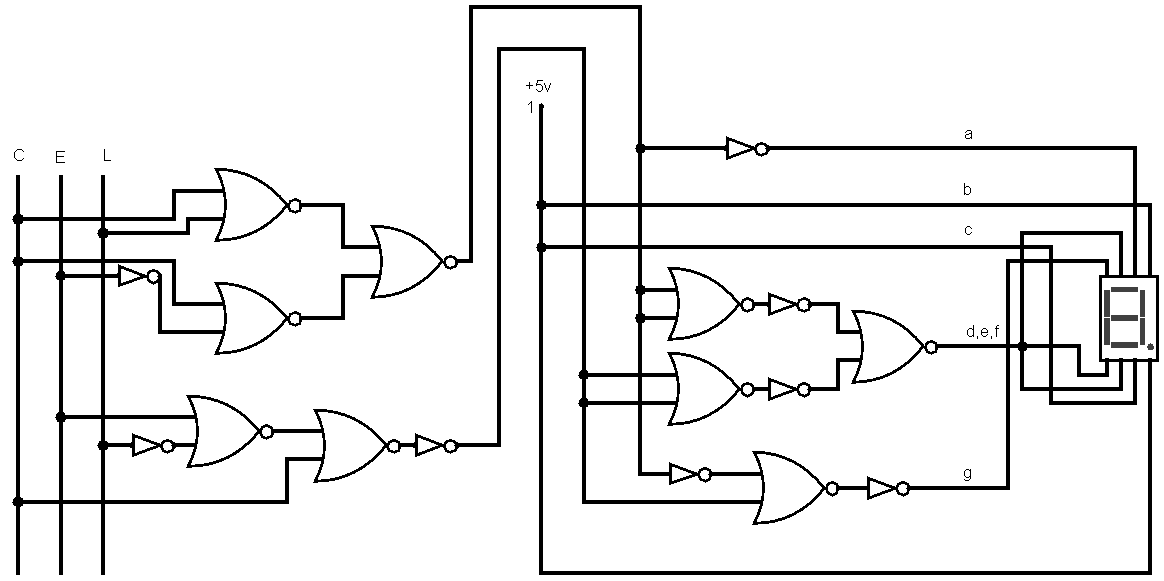
\includegraphics[width=14cm, keepaspectratio]{Final}\newline
\end{center}
Overall this lab went pretty smoothly, I was able to follow my prelab design pretty closely which allowed me to just focus on making sense of what was physically happening on my circuit. This lab was pretty enjoyable as I've always wanted to learn more about how 7-segment displays work.
\end{document}

